\documentclass[11pt]{article}
\usepackage{report}

\begin{document}
\section{Problem 1}
\subsection{Poisson}
For the poisson equation problem we have
\begin{align}
	-\nabla (a(x,y)\nabla u) &= f,\quad x\in \Omega \\
	u &= 0,\quad x\in \delta \Omega.
\end{align}
In order to rewrite this equation on weak, or variational, form we start with multiplying the integral of $f$ with a test function $v$ where $v\in V_0$ where $V_0 = \{ ||v||^2_{L^2} + ||\nabla v||^2 < \infty, v|_{\nabla \Omega} = 0\}$. This results in
\begin{align}
	\int_{\Omega} f v d s &= - \int_{\Omega} \nabla (a \nabla u) v ds \\
	&= \int_{\Omega} a \nabla u \nabla v ds - \int_{\delta \Omega} a v \nabla u d\bar{l} \\
	&= \int_{\Omega} a \nabla u \nabla v ds
\end{align}
where we used greens identity in the first step and the fact that the test function is zero at the boundary in the second step.
\subsection{Shroedinger}
When we look at the time dependent solution we have a significantly different problem.
\begin{align}
	\nabla^2 u + a(x,y) u &= f, \quad x\in \Omega \\
	u &= 0, \quad x \in \delta \Omega
\end{align}
We continue and do the same thing as we did for the poisson problem. Starting with multiplying the integral of f with a test function $v \in V_0$.
\begin{align}
	\int_{\Omega} f v d s &= - \int_{\Omega} \nabla^2 u v ds + \int_{\Omega} auv ds \\
	&= \int_{\Omega} \nabla u\nabla vds-\int_{\delta\Omega} v \nabla u d\bar{l} + \int_{\Omega} auvds \\
	&= \int_{\Omega} \nabla u \nabla v ds + \int_{\Omega} a u v ds
\end{align}
here the exact same steps as for the poisson derivation was made. The difference of course is the extra term $\int_{\Omega} a u v ds$ which is not within the derivate sign in the initial problem setup.

\section{Problem 2}
\subsection{Poisson}
In this problem we add some more complex boundary conditions. The poisson equation becomes 
\begin{align}
	-\Delta(a(x,y)\Delta u) &= f, \quad x\in\Omega \\
	c_0 u + c_1 \nabla u \cdot \hat{n} &= 0, \quad x \in\delta\Omega
\end{align}
We still use the same kind process of deriving the weak or variational form. One slight difference is that if u is gonna exists with in the test function space we need to change it a bit, so that it can be none zero at the boundary. Thus now we multiply the integral of f with a test function $v\in V_1$ where $V_1 = \{||v||^2_{L^2} + ||v'||^2_{L^2} < \infty\}$.
\begin{align}
	\int_{\Omega} f v ds &= - \int_{\Omega} \nabla (a\nabla u) ds \label{eq:poisGenVar}\\
	&= \int_{\Omega} a \nabla u \nabla v ds - \int_{\delta \Omega}a v \nabla u \cdot \hat{n} dl \\
	& = \int_{\Omega} a \nabla u \nabla v ds + \frac{c_0}{c_1}  \int_{\delta \Omega} a v u dl
\end{align}

\subsubsection{Energy norm}
For the energy norm we simply look at the variational form and make sure the terms including $u$ is on one side and take that side and put $v=u$ in order to get the an expression for the energy norm $||u||^2_E$
\begin{equation}
	||u||^2_E = \int_{\Omega} a (\nabla u)^2 ds + \frac{c_0}{c_1}  \int_{\delta \Omega} a u^2 dl
\end{equation}
This physically represents the energy in the system, while the left hand side of equation \ref{eq:poisGenVar} stands for the load on the system.

\subsection{Shroedinger}
Here we apply the same more complex boundary condidion to the time-independent shroedinger equation. 
\begin{align}
	\nabla^2 u + a(x,y) u &= f, \quad x\in \Omega \\
	c_0 u + c_1 \nabla u \cdot \hat{n} &= 0, \quad x \in \delta \Omega
\end{align}
And in order to get to the variational form we multiply the integral of f with a test function $v\in V_1$. 
\begin{align}
	\int_{\Omega} f v d s &= - \int_{\Omega} \nabla^2 u v ds + \int_{\Omega} auv ds \\
	&= \int_{\Omega} \nabla u\nabla vds-\int_{\delta\Omega} v \nabla u \cdot \hat{n}dl + \int_{\Omega} auvds \\
	&= \int_{\Omega} \nabla u \nabla v ds + \int_{\Omega} a u v ds + \frac{c_0}{c_1}\int_{\delta \Omega} u v dl 
\end{align}
\subsubsection{Energy norm}
For the energy norm we, again, look at the variational form and make sure the terms including $u$ is on one side and take that side and put $v=u$ in order to get the an expression for the energy norm $||u||^2_E$
\begin{equation}
	||u||^2_E = \int_{\Omega} (\nabla u)^2 ds + \int_{\Omega} a u^2 ds + \frac{c_0}{c_1}\int_{\delta \Omega} u^2 dl 
\end{equation}

\section{Problem 3}
In this exercise we wanna use the previous results and show how a finite elements approximation might look like. We will use the piecewise linear approximation. This means we will use a subspace of $V_0$ and $V_1$ which can be spanned by the hat functions, as define in the course book, that we will write as $\{\phi\}^{n_i}_{i=1}$.
\subsection{Poisson}
\subsubsection{Problem 1 Formulation}
We start off with
\begin{equation}
	\int_{\Omega} f v d s = \int_{\Omega} a \nabla u \nabla v ds
\end{equation}
Rewritting $v$ in terms of hat functions and we approximate $u$ as $u_h$ which is basically a solution projected onto the space spanned by the hat functions we get
\begin{equation}
	\int_{\Omega} f \phi_i ds = \sum^n_i \xi_i (\int_{\Omega} a \nabla \phi_i \nabla \phi_j ds)
\end{equation}
Which is what we where seeking.

\subsubsection{Problem 2 Forumlation}
In this exercise we do the same thing as in the previous but we have to take into account the extra terms given by the boundary conditions. We start off with
\begin{equation}
	\int_{\Omega} f v ds = \int_{\Omega} a \nabla u \nabla v ds + \frac{c_0}{c_1}  \int_{\delta \Omega} a v u dl.
\end{equation}
Doing the same thing to this expression as in the previous exercise we end up with
\begin{align}
	\int_{\Omega} f \phi_i ds &=  \sum^n_i \xi_i (\int_{\Omega} a \nabla \phi_i \nabla \phi_j ds) + \sum^n_i \frac{c_0}{c_1} \xi_i (\int_{\delta \Omega} a \phi_i \phi_j ds) \\
	&= \sum^n_i \xi_i ( \int_{\Omega} a \nabla \phi_i \nabla \phi_j ds + \frac{c_0}{c_1} \int_{\delta \Omega} a \phi_i \phi_j ds).
\end{align}
Here one has to care and realize that the last term in the expression is only on the boundary of the two dimensional geometry. 
\subsection{Shroedinger}
\subsubsection{Problem 1 Formulation}
In this exercise we start off with the variational formulation
\begin{equation}
	\int_{\Omega} fv ds= \int_{\Omega} \nabla u \nabla v ds + \int_{\Omega} a u v ds
\end{equation}
Using the subspace of $V_0$ that is spanned by the hat functions for the test function and solution space we get
\begin{align}
	\int_{\Omega} f \phi_i ds &= \sum^n_i \xi_i \int_{\Omega} \nabla \phi_i \nabla \phi_j ds + \sum^n_i \xi_i \int_{\Omega}a \phi_i \phi_j ds \\
	&= \sum^n_i \xi_i ( \int_{\Omega} \nabla \phi_i \nabla \phi_j ds + \int_{\Omega}a \phi_i \phi_j ds).
\end{align}
Here we can clearly see the use of both a stiffness matrix and a mass matrix. 

\subsubsection{Problem 2 Formulation}
Here we start of the variational forumalation
\begin{equation}
	\int_{\Omega} f v ds = \int_{\Omega} \nabla u \nabla v ds + \int_{\Omega} a u v ds + \frac{c_0}{c_1}\int_{\delta \Omega} u v dl 
\end{equation} 
Using the subspace of $V_0$ that is spanned by the hat functions for the test function and solution space we get
\begin{align}
	\int_{\Omega} f \phi_i ds &= \sum^n_i \xi_i \int_{\Omega} \nabla \phi_i \nabla \phi_j ds + \sum^n_i \xi_i \int_{\Omega} a \phi_i \phi_j  ds + \frac{c_0}{c_1} \sum^n_i \xi_i \int_{\delta \Omega} \phi_i \phi_j ds \\
	&= \sum^n_i \xi_i ( \int_{\Omega} \nabla \phi_i \nabla \phi_j ds + \int_{\Omega} a \phi_i \phi_j  ds + \frac{c_0}{c_1} \int_{\delta \Omega} \phi_i \phi_j ds )
\end{align}
Here we note we once again only get some extra terms on the boundary due to the more general formulation of the boundary conditions. 

\newpage
\section{Problem 4}
Here we implement a finite element solver for the Poisson equation within the unit square with $u=0$ on the boundary and $a=1$\footnote{Phew!}. We solve it with $f = 2 \pi^2 sin(\pi x) sin(\pi y)$. We have a mesh that goes between $h_{max} = 0.2,0.1,0.05,0,025$, this is depicted in figure \ref{fig:meshplot}.Using our implementation of the finite element method\footnote{all the code is attached in the appendix} We solve the system for every mesh and we get the result that is depicted in figure \ref{fig:ex4sol}. This could nicely be compared with the analytical solution to the problem in figure \ref{fig:anal}
\begin{figure}[H]
	\centering
	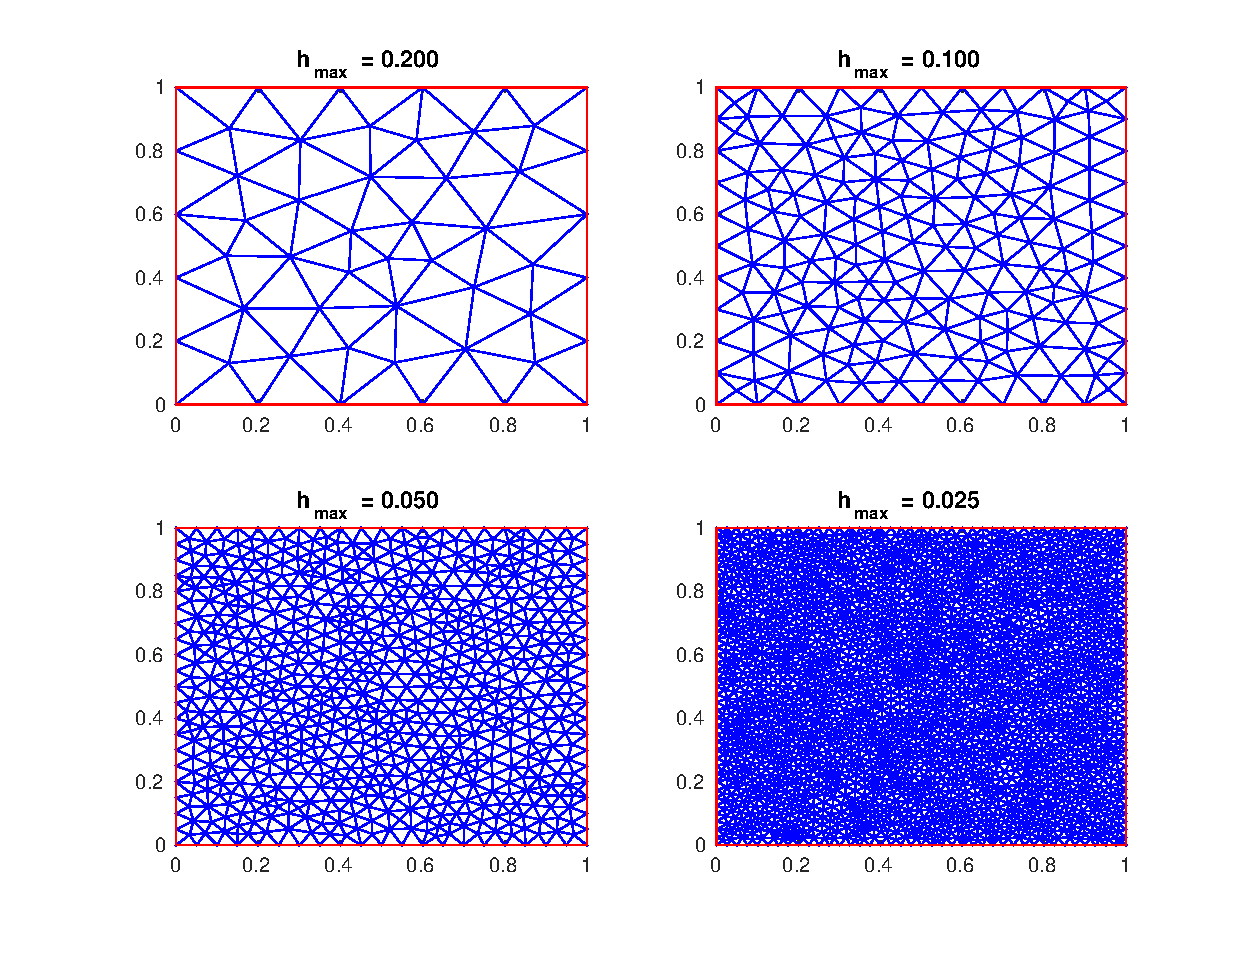
\includegraphics[width=1\textwidth]{../ex4/meshplot}
	\caption{Here we see the different meshes we are working on}
	\label{fig:meshplot}
\end{figure}
\begin{figure}[H]
	\centering
	\includegraphics[width=1\textwidth]{../ex4/sol}
	\caption{The numerical ssolution to the system we are looking at, the figures looks uggly since matlab is horrid at exporting and presenting data in a halfdeacent format.}
	\label{fig:ex4sol}
\end{figure}
\begin{figure}[H]
	\centering
	\includegraphics[width=1\textwidth]{../ex4/anal}
	\caption{The analytical solution to the system we are looking at, the figures looks uggly since matlab is horrid at exporting and presenting data in a halfdeacent format.}
	\label{fig:anal}
\end{figure}
But perhaps the smartest way of doing it is to look at the energy norm of the error for the system. The errror is depicted in figure \ref{fig:ex4error}. Something of interest here is the convergence of the system. The convergence is the $s$ in the equation
\begin{equation}
	||u-u_h||^2_E \leq c h^s.
	\label{eq:errorBounds}
\end{equation}
Using this we can analytically solve the equation and get a lower bound for the $s$. Using the fact that 
\begin{equation}
	||u-u_h||^2_E = ||u||^2 - ||u_h||^2 \leq c h^s \label{eq:error}
\end{equation}
we can calculate two errors and divide the resulting equation to end up with 
\begin{align}
	ln(\frac{e_1}{e_2}) &\leq s ln(\frac{h_1}{h_2}) \\
	s &\geq \frac{ln(\frac{e_1}{e_2})}{ln(\frac{h_1}{h_2})} \label{eq:findS}
\end{align}
Using this we can calculate $s$ analytically and do a fitting of a log plot of step size vs energy norm of the error. As expected we find that the fitted value for $s$ is sligtly larger then the calculated one. This since the calculated one is the lowest possible value that $s$ should be able to take. As expected from theory this value is very close to one. One can discuss why the measured error is not straight. This is because the $c$ in equation \ref{eq:ex4error} is not completly constant but has a dependency on how different the chunkiness are for different triangels in the mesh. 
\begin{figure}[H]
	\centering
	\includegraphics[width=1\textwidth]{../ex4/error}
	\caption{The energy norm of the error in the system we solved for different $h_{max}$}
	\label{fig:ex4error}
\end{figure}

\section{Problem 5}
Here we do the same thing as in the previous exercise, with the same analysis done and same size meshes. Difference is that we do it for the shroedinger problem with $u=0$ and $a=1$. The only interessting pitfalls is that you have ho assemble a slightly different system matrix for this problem using both the stiffness and mass matrix.The code is attached in the appendix.

\begin{figure}[H]
	\centering
	\includegraphics[width=1\textwidth]{../ex5/sol}
	\caption{The numerical ssolution to the system we are looking at, the figures looks uggly since matlab is horrid at exporting and presenting data in a halfdeacent format.}
	\label{fig:ex5sol}
\end{figure}
\begin{figure}[H]
	\centering
	\includegraphics[width=1\textwidth]{../ex5/error}
	\caption{The energy norm of the error in the system we solved}
	\label{fig:ex5error}
\end{figure}

\newpage
\appendix
\section{code: Problem 4}
\subsection{solve.m}
\verbatimtabinput{../ex4/solve.m}
\subsection{loadAssembler.m}
\verbatimtabinput{../ex4/loadAssembler.m}
\subsection{systemMatrixAssembler.m}
\verbatimtabinput{../ex4/systemMatrixAssembler.m}

\section{code: Problem 5}
\subsection{solve.m}
\verbatimtabinput{../ex5/solve.m}
\subsection{loadAssembler.m}
\verbatimtabinput{../ex5/loadAssembler.m}
\subsection{systemMatrixAssembler.m}
\verbatimtabinput{../ex5/systemMatrixAssembler.m}



\end{document}

